\section{Experimental Evaluation}
\label{sec:results}
% Numerical source: main0928/had/aggregates.json, paper1007.
% R=-D. SD is sample SD (ddof=1); learning-method unit is training seed.
% The optional full-variant macro is placed by main.tex in its existing appendix.

\newcommand{\HadMainTable}{%
\begin{table*}[!t]
\centering\footnotesize
\setlength{\tabcolsep}{5pt}
\caption{Formal HAD comparison: mean $\pm$ sample SD. Reward $R=-D$ is higher-is-better; friendly-collision mortality $C$ is lower-is-better. Each learned method has three training seeds and 300 common scenes per configuration. Bold marks the best group mean for each metric.}
\label{tab:had-main}
\begin{tabular*}{\textwidth}{@{\extracolsep{\fill}}llrrrr@{}}
\toprule
Method & Metric & ID & $K$-OOD & $N$-OOD & Joint OOD \\
\midrule
\textbf{LEAF} & $R\uparrow$ & $\mathbf{-0.405\pm0.097}$ & $\mathbf{-0.996\pm0.233}$ & $\mathbf{-0.575\pm0.235}$ & $\mathbf{-1.097\pm0.105}$ \\
 & $C\downarrow$ (\%) & $\mathbf{1.33\pm0.45}$ & $\mathbf{1.70\pm0.62}$ & $6.29\pm1.32$ & $4.97\pm1.26$ \\
\addlinespace[2pt]
REFIL & $R\uparrow$ & $-0.715\pm0.049$ & $-1.796\pm0.304$ & $-2.209\pm0.277$ & $-3.308\pm0.303$ \\
 & $C\downarrow$ (\%) & $2.97\pm0.42$ & $4.71\pm0.67$ & $12.86\pm2.14$ & $10.34\pm1.69$ \\
\addlinespace[2pt]
QMIX-Atten & $R\uparrow$ & $-2.318\pm1.431$ & $-5.009\pm2.497$ & $-5.139\pm3.111$ & $-7.415\pm3.970$ \\
 & $C\downarrow$ (\%) & $10.82\pm9.56$ & $12.42\pm9.75$ & $16.38\pm5.43$ & $15.37\pm7.34$ \\
\addlinespace[2pt]
DCG & $R\uparrow$ & $-2.028\pm0.437$ & $-5.839\pm1.920$ & $-5.021\pm2.658$ & $-8.092\pm3.909$ \\
 & $C\downarrow$ (\%) & $9.05\pm3.36$ & $14.97\pm4.68$ & $19.70\pm8.52$ & $19.26\pm10.20$ \\
\addlinespace[2pt]
SPECTra & $R\uparrow$ & $-2.662\pm0.070$ & $-6.933\pm0.670$ & $-6.455\pm1.403$ & $-11.184\pm0.352$ \\
 & $C\downarrow$ (\%) & $13.06\pm0.75$ & $20.71\pm1.60$ & $28.92\pm1.54$ & $31.25\pm1.63$ \\
\addlinespace[2pt]
ALMA & $R\uparrow$ & $-1.326\pm0.193$ & $-3.022\pm0.344$ & $-3.605\pm0.742$ & $-5.375\pm1.036$ \\
 & $C\downarrow$ (\%) & $7.42\pm1.13$ & $9.05\pm1.66$ & $18.42\pm3.84$ & $15.92\pm3.86$ \\
\addlinespace[2pt]
Rule$^{\dagger}$ & $R\uparrow$ & $-1.462\pm0.717$ & $-3.212\pm1.126$ & $-1.545\pm0.881$ & $-3.060\pm0.976$ \\
 & $C\downarrow$ (\%) & $1.98\pm4.47$ & $2.70\pm3.57$ & $\mathbf{5.70\pm3.30}$ & $\mathbf{4.48\pm2.44}$ \\
\bottomrule
\end{tabular*}
\par\vspace{2pt}\parbox{\textwidth}{\footnotesize
$\dagger$ Rule has no training seeds. Its SD is across the 300 scene seeds, after averaging configurations within each scene. All other SDs measure training-seed variation. Collision SDs are percentage points.}
\end{table*}}

\newcommand{\HadCoreAblationTable}{%
\begin{table*}[!t]
\centering\footnotesize
\setlength{\tabcolsep}{5pt}
\caption{Core design references on the formal HAD matrix: absolute reward $R=-D$ and friendly-collision mortality $C$, mean $\pm$ sample SD across three training seeds. Each configuration uses 300 common scenes. Bold marks the best mean among these five methods. SG denotes + Memory query; NoREFIL, R0, and R1 retain historical-query inputs.}
\label{tab:had-core-ablation}
\begin{tabular*}{\textwidth}{@{\extracolsep{\fill}}llrrrr@{}}
\toprule
Method & Metric & ID & $K$-OOD & $N$-OOD & Joint OOD \\
\midrule
\textbf{LEAF} & $R\uparrow$ & $\mathbf{-0.405\pm0.097}$ & $\mathbf{-0.996\pm0.233}$ & $\mathbf{-0.575\pm0.235}$ & $\mathbf{-1.097\pm0.105}$ \\
 & $C\downarrow$ (\%) & $\mathbf{1.33\pm0.45}$ & $\mathbf{1.70\pm0.62}$ & $\mathbf{6.29\pm1.32}$ & $\mathbf{4.97\pm1.26}$ \\
\addlinespace[2pt]
SG (+ Memory query) & $R\uparrow$ & $-0.527\pm0.227$ & $-1.529\pm0.734$ & $-0.998\pm0.621$ & $-1.946\pm1.229$ \\
 & $C\downarrow$ (\%) & $1.66\pm0.86$ & $2.59\pm1.78$ & $8.57\pm4.41$ & $6.65\pm4.16$ \\
\addlinespace[2pt]
NoREFIL & $R\uparrow$ & $-0.510\pm0.138$ & $-1.768\pm0.621$ & $-1.263\pm0.653$ & $-2.319\pm0.889$ \\
 & $C\downarrow$ (\%) & $2.23\pm0.77$ & $3.67\pm1.65$ & $10.71\pm3.98$ & $8.76\pm3.14$ \\
\addlinespace[2pt]
R0 & $R\uparrow$ & $-0.928\pm0.210$ & $-1.958\pm0.457$ & $-2.020\pm0.446$ & $-3.196\pm0.687$ \\
 & $C\downarrow$ (\%) & $3.34\pm1.66$ & $4.46\pm2.10$ & $11.16\pm1.81$ & $9.17\pm2.18$ \\
\addlinespace[2pt]
1-round (R1) & $R\uparrow$ & $-0.609\pm0.272$ & $-1.203\pm0.402$ & $-1.355\pm0.884$ & $-2.157\pm1.006$ \\
 & $C\downarrow$ (\%) & $1.57\pm0.15$ & $2.08\pm0.32$ & $8.35\pm3.16$ & $6.56\pm2.37$ \\
\bottomrule
\end{tabular*}
\par\vspace{2pt}\parbox{\textwidth}{\footnotesize
Groups weight configurations equally within each training seed. All SDs measure training-seed variation; collision SDs are percentage points. These are absolute results for complete trained designs, with the paired design questions explained in the text.}
\end{table*}}

\newcommand{\HadFullVariantTable}{%
\begin{table*}[!t]
\centering\footnotesize
\setlength{\tabcolsep}{4pt}
\caption{All ten completed main0928 design variants on the same formal matrix: reward mean $\pm$ sample SD across three training seeds. These results retain the context in which LEAF was selected. Comparison variants beyond + Memory query also change architecture or training/execution choices.}
\label{tab:had-full-variants}
\begin{tabular*}{\textwidth}{@{\extracolsep{\fill}}lrrrr@{}}
\toprule
Method & ID & $K$-OOD & $N$-OOD & Joint OOD \\
\midrule
\textbf{LEAF} & $-0.405\pm0.097$ & $-0.996\pm0.233$ & $-0.575\pm0.235$ & $-1.097\pm0.105$ \\
+ Memory query & $-0.527\pm0.227$ & $-1.529\pm0.734$ & $-0.998\pm0.621$ & $-1.946\pm1.229$ \\
NoREFIL & $-0.510\pm0.138$ & $-1.768\pm0.621$ & $-1.263\pm0.653$ & $-2.319\pm0.889$ \\
R0 & $-0.928\pm0.210$ & $-1.958\pm0.457$ & $-2.020\pm0.446$ & $-3.196\pm0.687$ \\
1-round & $-0.609\pm0.272$ & $-1.203\pm0.402$ & $-1.355\pm0.884$ & $-2.157\pm1.006$ \\
Last & $-0.434\pm0.083$ & $-1.020\pm0.100$ & $-0.652\pm0.160$ & $-1.269\pm0.202$ \\
Fixed4 & $-0.407\pm0.204$ & $-1.004\pm0.665$ & $-0.659\pm0.184$ & $-1.265\pm0.230$ \\
ARR & $-0.469\pm0.091$ & $-1.221\pm0.344$ & $-1.778\pm1.292$ & $-2.370\pm1.164$ \\
Untied4 & $-0.476\pm0.183$ & $-1.127\pm0.157$ & $-0.543\pm0.156$ & $-1.232\pm0.253$ \\
Looped + count & $-0.596\pm0.145$ & $-1.301\pm0.427$ & $-1.075\pm0.449$ & $-1.685\pm0.844$ \\
\bottomrule
\end{tabular*}
\end{table*}}


\noindent\textbf{Setup and statistics.}
We evaluate HAD target protection against a fixed reactive--rush attacker, using public physical entity states and a horizon of 100 environment steps. Training samples balanced teams $N_R=N_B=N\in\{4,6,8,10\}$ and target counts $K\in\{1,2,3\}$. Each learned method has three training seeds and a nominal budget of $10^6$ physical environment steps per seed. LEAF retains the REFIL host and downstream GRU, uses a self-conditioned relation query without previous GRU state, disables explicit count injection, samples one through four relation rounds during training, and executes four rounds for formal evaluation. Hidden width is 64, with four attention heads, learning rate $5\times10^{-4}$, discount 0.99, batch size 32, and replay capacity 5000.

Frozen final checkpoints are evaluated on 24 configurations, with 300 common scene seeds (9000--9299) per configuration. ID comprises $(4,4,2)$, $(6,6,2)$, $(8,8,2)$, and $(10,10,3)$. $K$-OOD uses $(10,10,K)$ for $K\in\{4,6,9,12\}$; $N$-OOD uses $(N,N,2)$ for $N\in\{15,20,25,30,40,50\}$. Joint OOD combines $N\in\{15,20,30\}$ with $K\in\{4,6\}$ and adds $(30,30,9)$ and $(30,30,12)$. Supporting configurations are $(5,5,2)$ and $(10,10,2)$. The learned baselines are REFIL, QMIX-Atten, DCG, SPECTra, and ALMA; Rule is a fixed policy. Historical baseline checkpoints and their evaluation slices are reused with their recorded identities and interaction budgets.

The primary metric is unshaped episode reward $R=-D$, with higher values indicating better protection. The second metric is friendly-collision mortality,
\begin{equation}
 C=\frac{\text{defenders killed by friendly collision}}{N_R},
\end{equation}
with lower values preferred. Each training seed first averages the 300 scenes within a configuration and then weights configurations equally within a group. We report mean $\pm$ sample standard deviation (SD) across the three trained models. For Rule, configurations are averaged within each common scene seed before computing SD across 300 scene seeds. These SDs describe different sources of variation and are not confidence intervals~\cite{agarwal2021rliable}.

Training validation uses 50 checkpoints and the same four ID configurations, with 25 fixed scenes per configuration in seed blocks spanning 9500--9599. Curves align evaluation indices, average configurations within each training seed, and show the three-seed mean and sample SD at the mean recorded environment step count, without smoothing. Validation scenes differ from the 300-scene formal evaluation pool, so the last curve point need not equal the ID value in the formal tables.

\subsection{Comparison Across Deployment Populations}
\label{subsec:comparison}
Table~\ref{tab:had-main} shows the highest group mean reward for LEAF among the six learned methods and Rule in all four groups. Relative to REFIL, its reward improves by 0.310, 0.800, 1.635, and 2.211 in ID, $K$-OOD, $N$-OOD, and Joint OOD. Each improvement holds in all three corresponding training-seed comparisons. Figure~\ref{fig:had-generalization} shows validation during training separately from target-count, team-size, and joint transfer of frozen final checkpoints.

At validation checkpoint 10 (approximately $0.2$ million steps), LEAF has reward $-2.046\pm0.028$ versus REFIL's $-4.429\pm0.284$. At checkpoint 50, the values are $-0.373\pm0.066$ and $-0.738\pm0.122$. These observations describe the recorded ID learning trajectories; they do not establish an improvement for every checkpoint or a general sample-efficiency claim.

LEAF has lower mean collision mortality than every learned baseline in each group. Rule has lower mortality in $N$-OOD (5.70\% versus 6.29\%) and Joint OOD (4.48\% versus 4.97\%), despite lower reward. Minimizing friendly losses alone therefore does not explain target protection.

\HadMainTable

\begin{figure*}[!t]
\centering
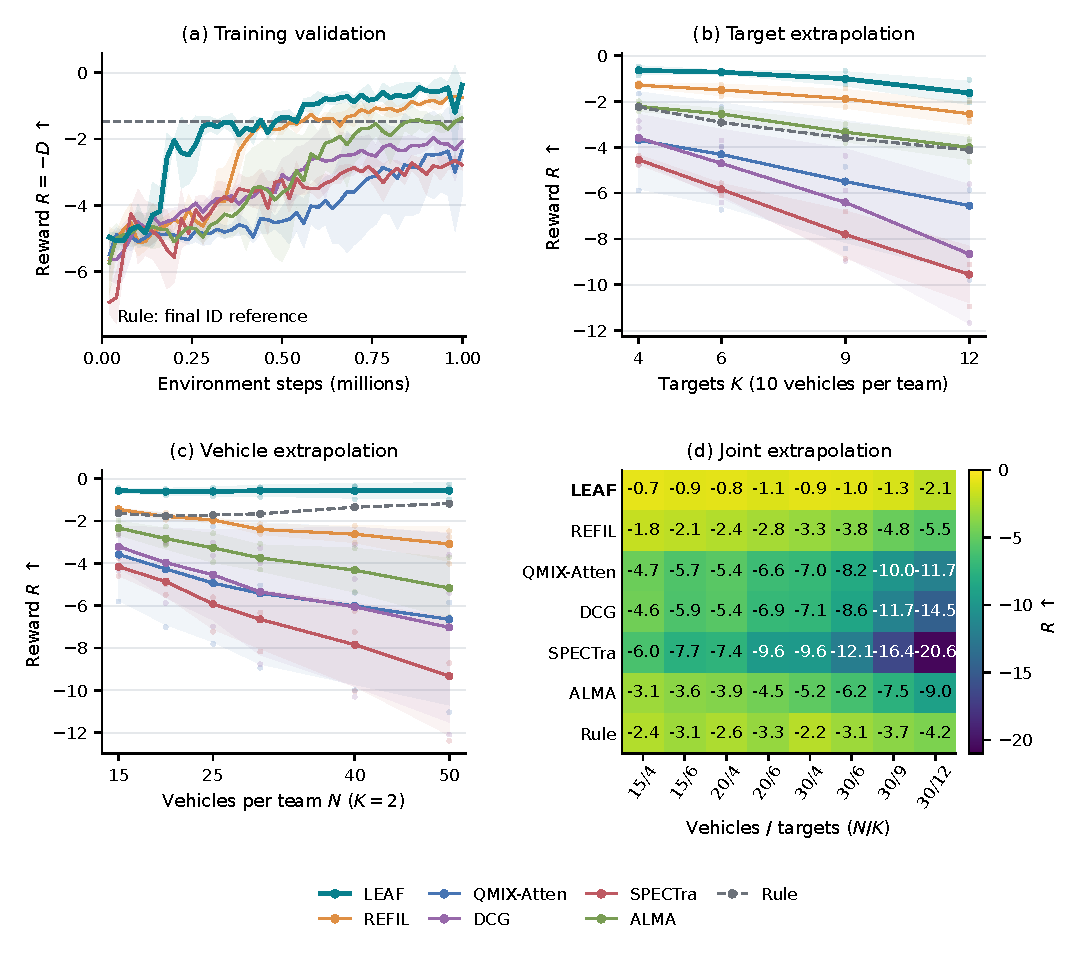
\includegraphics[width=\textwidth]{figures/fig_had_generalization.pdf}
\caption{Learning and formal generalization. (a) Fifty native validation checkpoints for LEAF and the five learned baselines, plotted at actual mean environment steps without smoothing; bands show one training-seed sample SD. Validation uses fixed scene seeds 9500--9599; Rule is a formal final-ID reference. (b)--(c) Target-count and team-size transfer retain seed points and SD bands. (d) All eight Joint OOD configurations share a linear reward scale. Learning-record sources are described in Appendix~\ref{app:learning-source}.}
\label{fig:had-generalization}
\end{figure*}

\subsection{Ablation and Design Comparisons}
\label{subsec:ablation}
Table~\ref{tab:had-core-ablation} reports absolute reward and collision mortality for the five core design references across all four groups. Figure~\ref{fig:had-ablation} complements those endpoints with validation during training and transfer along the target, vehicle, and joint population axes. The design study addresses three paired questions. First, does contextual entity processing help before reading? Within the historical-query branch, R0 reads the original entity representations, whereas 1-round (R1) performs one contextual update. R1 improves mean reward by 0.319, 0.755, 0.665, and 1.039 across ID, $K$-OOD, $N$-OOD, and Joint OOD, respectively. Two of three seed pairs improve in each group. This comparison supports developing entity context before the readout.

Second, does the relation query need an additional GRU-history input? The closest contrast to LEAF restores detached GRU history in that query, denoted \emph{+ Memory query} (the historical SG variant). Both policies retain downstream recurrence and previous-action input features. Removing GRU history from the query gives LEAF mean reward gains of 0.122, 0.533, 0.424, and 0.849 across the four groups, with agreement in all three ID seeds and two of three seeds per OOD group. This favors self-conditioned reading with temporal memory downstream at the group-mean level. Frozen GRU intervention below examines whether the saved LEAF policy actually depends on that downstream memory.

Third, how does the relational path work with its host? NoREFIL removes the local host, imagination paths, and associated losses while retaining a historical query. Restoring this bundle gives SG higher mean reward in the three extrapolation groups by 0.239, 0.265, and 0.372, with a slight ID decrease of 0.017. This is a whole-architecture contrast; it does not isolate the contribution of any one removed path or loss. Together, the three comparisons examine contextual processing, memory placement, and host integration without treating all variants as single-component deletions from LEAF.

\HadCoreAblationTable

\begin{figure*}[!t]
\centering
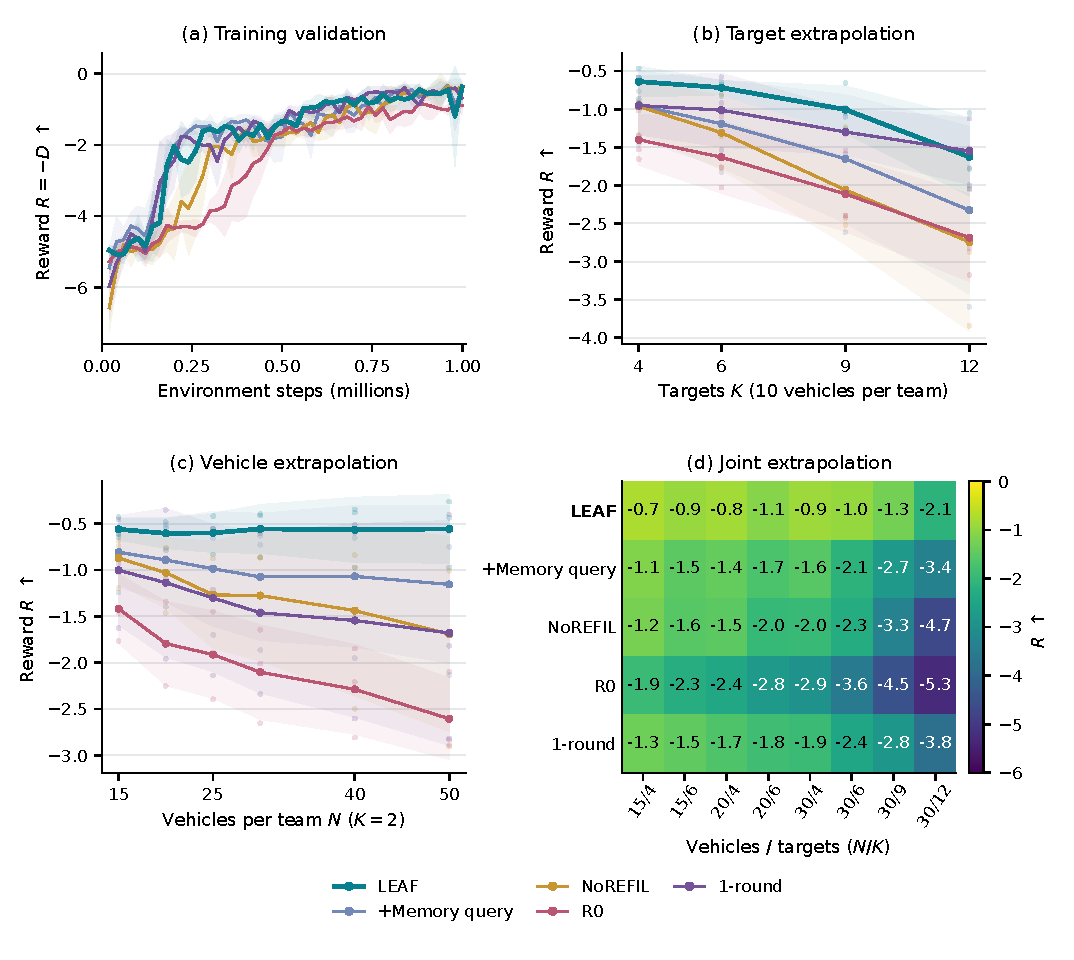
\includegraphics[width=\textwidth]{figures/fig_had_ablation.pdf}
\caption{Validation and population transfer for LEAF, SG (+ Memory query), NoREFIL, R0, and 1-round (R1). (a) Fifty validation checkpoints aligned by evaluation index, with actual mean environment steps on the horizontal axis and mean $\pm$ sample SD across three training seeds; no smoothing is applied. (b)--(c) Absolute reward under target-count and vehicle-count extrapolation, retaining seed points and SD bands. (d) All eight Joint OOD configurations use one linear reward scale, with cell means rounded for display. SG, NoREFIL, R0, and R1 use historical queries. NoREFIL to SG restores the local host, imagination paths, and associated losses together. The text distinguishes the three paired design questions from complete-design comparisons with LEAF and from frozen execution interventions.}
\label{fig:had-ablation}
\end{figure*}

NoREFIL, R0, and R1 are complete-design references when compared directly with LEAF because they also use a historical query. QMIX-Atten and REFIL provide external and host references in Table~\ref{tab:had-main}. A capacity control, REFIL-matched, has 176,393 actor parameters versus LEAF's 175,754 (a 0.36\% difference) and REFIL's 102,025. Its group reward means are $-0.914$, $-2.493$, $-2.269$, and $-4.170$; LEAF improves each in all three seed pairs. This weakens a parameter-count-only explanation, while leaving architecture and optimization differences coupled.

Similar ID validation endpoints do not guarantee similar transfer: NoREFIL's last validation reward is $-0.381\pm0.126$, close to LEAF's $-0.373\pm0.066$, but its formal OOD group means are lower. Group means also do not imply superiority at every configuration: at $(10,10,12)$, R1 has reward $-1.548\pm0.439$ versus LEAF's $-1.625\pm0.515$.

LEAF was selected after inspecting ten completed variants on the formal matrix. Table~\ref{tab:had-full-variants} preserves that selection context. Increasing beyond one round does not improve every group, and learned fusion, depth sampling, and parameter sharing give mixed trained-design results. These choices remain part of the evaluated architecture rather than separate improvement claims. Untied4 has a higher $N$-OOD reward mean than LEAF ($-0.543$ versus $-0.575$); LEAF is higher in the other groups.

\subsection{Mechanism: Looped Context, Fusion, and Memory}
\label{subsec:mechanism}
\noindent\textbf{Protocol.}
Frozen interventions use three registered LEAF final checkpoints at $(10,10,2)$, $(50,50,2)$, and $(30,30,12)$ on common scenes 9000--9009, without weight updates. Eight execution changes examine one or two rounds, reading original tokens $H^{(0)}$ without contextual updates, final-read-only fusion, uniform fusion, fixed mean fusion, zero relation residual, and GRU reset. The $H^{(0)}$ control preserves the self query, read attention, residual projection, local host, and GRU. Residual zeroing removes the complete projection including its bias; GRU reset retains previous-action features.

For fixed fusion, each model's factual fusion weights are averaged over live decisions within each configuration, then equally over the three configurations. These four nonuniform weights replace state-dependent scores at every decision; all four contextual updates and reads remain. This is a diagnostic mean computed on the same scene pool, without reward optimization or a held-out calibration claim.

Closed-loop reward changes are paired with a local standard execution within scene and model seed, averaged over ten scenes, then summarized across three seeds. Same-state forwards separately reuse standard entities, previous actions, and incoming GRU state, restoring factual hidden state, cached values, and random state before the rollout continues. Action-change rates count live defender decisions. The study executed 990 episodes: the original 720, plus 90 standard recaptures and 180 new loop/fusion controls. All 90 recaptures match the earlier local standard in 11 fields. Historical comparison has a narrower agreement range (Appendix~\ref{app:replay}), so these diagnostics do not replace formal performance estimates.

\noindent\textbf{Looped processing builds decision-relevant context.}
Reading $H^{(0)}$ without the loop changes 69.62--72.41\% of same-state greedy actions. Relative to standard LEAF, reward changes by $-7.556\pm1.365$, $-18.962\pm5.828$, and $-32.968\pm8.447$ in the configuration order above; all nine model--configuration means decrease. The R0--R1 trained-design contrast in Section~\ref{subsec:ablation} favors one contextual update, and this direct frozen control establishes that LEAF's learned policy relies on the resulting context. Together they support entity processing before reading. They do not establish that four updates are necessary: two-round reward changes are $-0.273\pm0.047$, $0.001\pm0.205$, and $0.264\pm1.259$, respectively.

\noindent\textbf{Fusion favors early context, with conditional later-read sensitivity.}
The first two rounds receive 98.59--98.91\% of average fusion weight. Forcing the final read, using uniform fusion, or zeroing the relation projection reduces reward in all nine model--configuration means (Fig.~\ref{fig:had-mechanism}). These interventions show reliance on access to the learned intermediate features, but do not alone establish the benefit of state-dependent weights over a fixed shallow preference.

The fixed mean control makes that distinction: it changes 9.88--10.54\% of same-state actions, yet reward changes are $0.006\pm0.109$, $0.092\pm0.121$, and $-0.612\pm0.471$. Its effect is mixed across models at the two $K=2$ configurations, whereas all three models lose reward at $(30,30,12)$. Thus state-dependent fusion has consistent local support in the target-rich case; a broad dynamic-fusion advantage is not established. The strongest shared finding is selective use of early contextual reads.

Later reads still affect a small subset of decisions. Of 48,705 factual live-defender decisions, two-round execution changes 753 actions. Within every model--configuration group, changed decisions have smaller average standard Q margins and larger late-round weights than unchanged decisions. Approximately 78.63\%, 80.88\%, and 78.30\% of changes fall in the lowest-margin decile of their respective groups, averaged equally over model seeds (Fig.~\ref{fig:fusion-sensitivity}). Equation~\eqref{eq:depth-perturbation} relates late weight to the projected feature change; Eq.~\eqref{eq:greedy-stability} explains why small perturbations can matter near an action boundary. Its sufficient condition covers 78.56--83.76\% of decisions, all with unchanged actions. This reconciles shallow weight concentration with local later-read sensitivity, without assigning every changed action a beneficial reward effect.

\noindent\textbf{Temporal memory and protective outcomes complete the account.}
Resetting downstream GRU state changes 58.37--62.90\% of same-state actions and decreases reward in eight of nine model--configuration means; seed 0 at $(30,30,12)$ is the exception. This complements the SG--LEAF comparison: omitting historical input from the query leaves a useful temporal role downstream. At $(50,50,2)$ in the formal 300-scene evaluation, LEAF has collision mortality $11.14\%\pm2.63\%$ versus REFIL's $19.59\%\pm3.69\%$, attacker interception $78.68\%\pm1.39\%$ versus $72.27\%\pm0.77\%$, and any-target-damage incidence $28.11\%\pm15.03\%$ versus $70.56\%\pm7.65\%$. These outcomes associate higher reward with effective protection. A separate common 100-scene arm finds higher geometric pursuit overlap for LEAF ($43.93\%\pm4.20\%$ versus $35.49\%\pm1.50\%$), so uniformly reducing duplicate pursuit is not the explanation. The overlap measure counts attackers pursued by at least two defenders within 1500\,m and a $30^\circ$ velocity cone; it does not label allocation errors.

\begin{figure*}[!t]
\centering
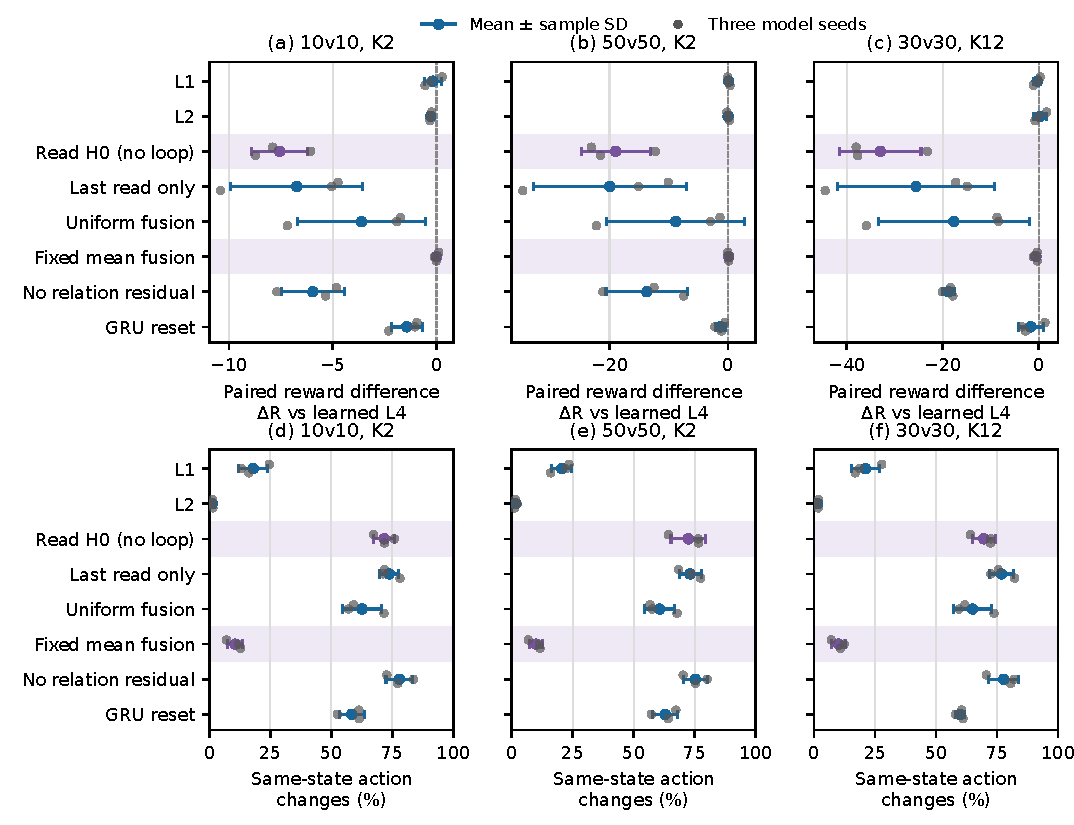
\includegraphics[width=\textwidth]{figures/fig_leaf_final1007_mechanism.pdf}
\caption{Eight frozen-final LEAF interventions on three configurations and ten common scenes per model seed. Top: reward change relative to local standard four-round fusion; positive values favor the intervention. Bottom: same-state greedy-action changes. Points and bars show three-model mean and sample SD; small points retain each model. Shaded loop/fixed-fusion controls use the new runtime, with remaining arms from the original runtime; each is paired with its own local standard (Appendix~\ref{app:replay}). Frozen execution dependence differs from retrained design effects.}
\label{fig:had-mechanism}
\end{figure*}

\begin{figure*}[!t]
\centering
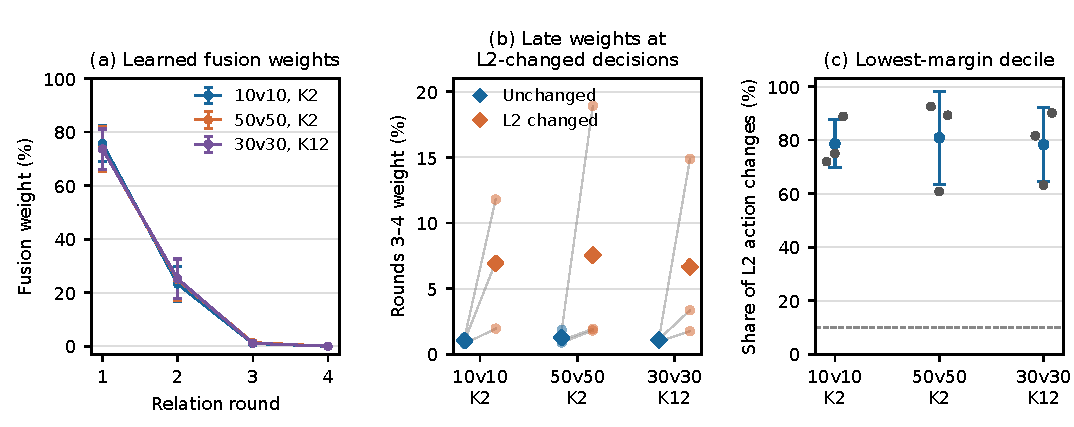
\includegraphics[width=\textwidth]{figures/fig_leaf_fusion_sensitivity.pdf}
\caption{Early-read preference and conditional later-read sensitivity on 90 standard LEAF trajectories. (a) Mean fusion weights with model-seed sample SD. (b) Late-round weight among decisions whose actions change under L2 versus those unchanged: small connected points pair each model; diamonds show the three-model mean. (c) Fraction of L2 action changes in the lowest Q-margin decile within each model and configuration; bars show model-seed SD and the dashed line marks 10\%. These local diagnostics describe decision sensitivity, not the direction of closed-loop reward effects.}
\label{fig:fusion-sensitivity}
\end{figure*}

\subsection{Representative Trajectories}
\label{subsec:trajectories}
Figure~\ref{fig:had-cases} compares LEAF, the five learned baselines, and Rule at $(5,5,2)$ and $(15,15,2)$. The learned policies use registered final checkpoints with training seed 0; both configurations use the preselected scene seed 9000. Initial physical states are identical across all seven methods within each configuration. A common snapshot at physical step 30 shows approach paths and surviving entities, while the adjacent reward plot follows each complete episode to its actual termination.

At 5v5, LEAF, REFIL, and ALMA each finish with reward $-1$, so this scene does not establish a unique LEAF advantage. At 15v15, LEAF prevents target damage and terminates at step 35; REFIL, QMIX-Atten, DCG, SPECTra, ALMA, and Rule receive $-5$, $-6$, $-7$, $-5$, $-1$, and $-1$, respectively. The panels connect movement and interception to the timing of target damage under a shared initial layout. These illustrative cases do not replace the 300-scene population statistics. Eleven of the fourteen local replays match all archived comparison fields; the remaining differences are retained in Appendix~\ref{app:replay}.

\begin{figure*}[!t]
\centering
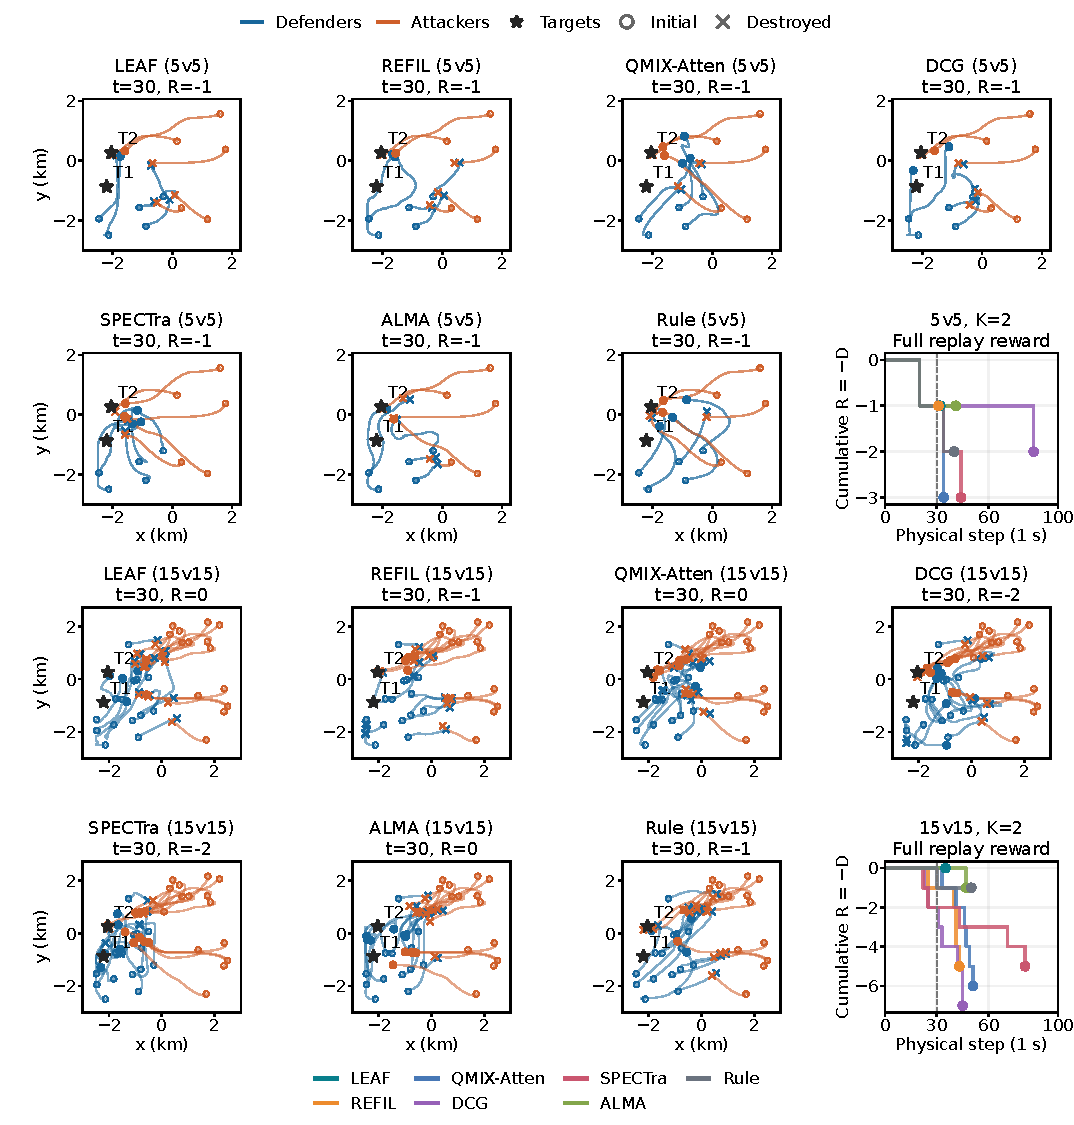
\includegraphics[width=\textwidth]{figures/fig_leaf_final1007_trajectory.pdf}
\caption{Seven-method trajectories on preselected scene 9000: the upper two rows show 5v5 and the lower two rows show 15v15, both with two targets. Each block contains seven spatial panels and a shared cumulative-reward plot. Learned policies use final checkpoints from training seed 0. Paths end at the common snapshot step 30; open circles show initial positions, filled circles show live vehicles, crosses show destroyed vehicles, and stars show targets. Spatial titles give reward at the snapshot. Reward curves continue to each actual terminal step, marked by a dot; the dashed line marks the snapshot. Entity colors and spatial limits are shared within each scale.}
\label{fig:had-cases}
\end{figure*}
